\section{RRTExt\-Ext  Class Reference}
\label{classRRTExtExt}\index{RRTExtExt@{RRTExt\-Ext}}
Balance between growing trees toward each other and exploring. 


{\tt \#include $<$rrt.h$>$}

Inheritance diagram for RRTExt\-Ext::\begin{figure}[H]
\begin{center}
\leavevmode
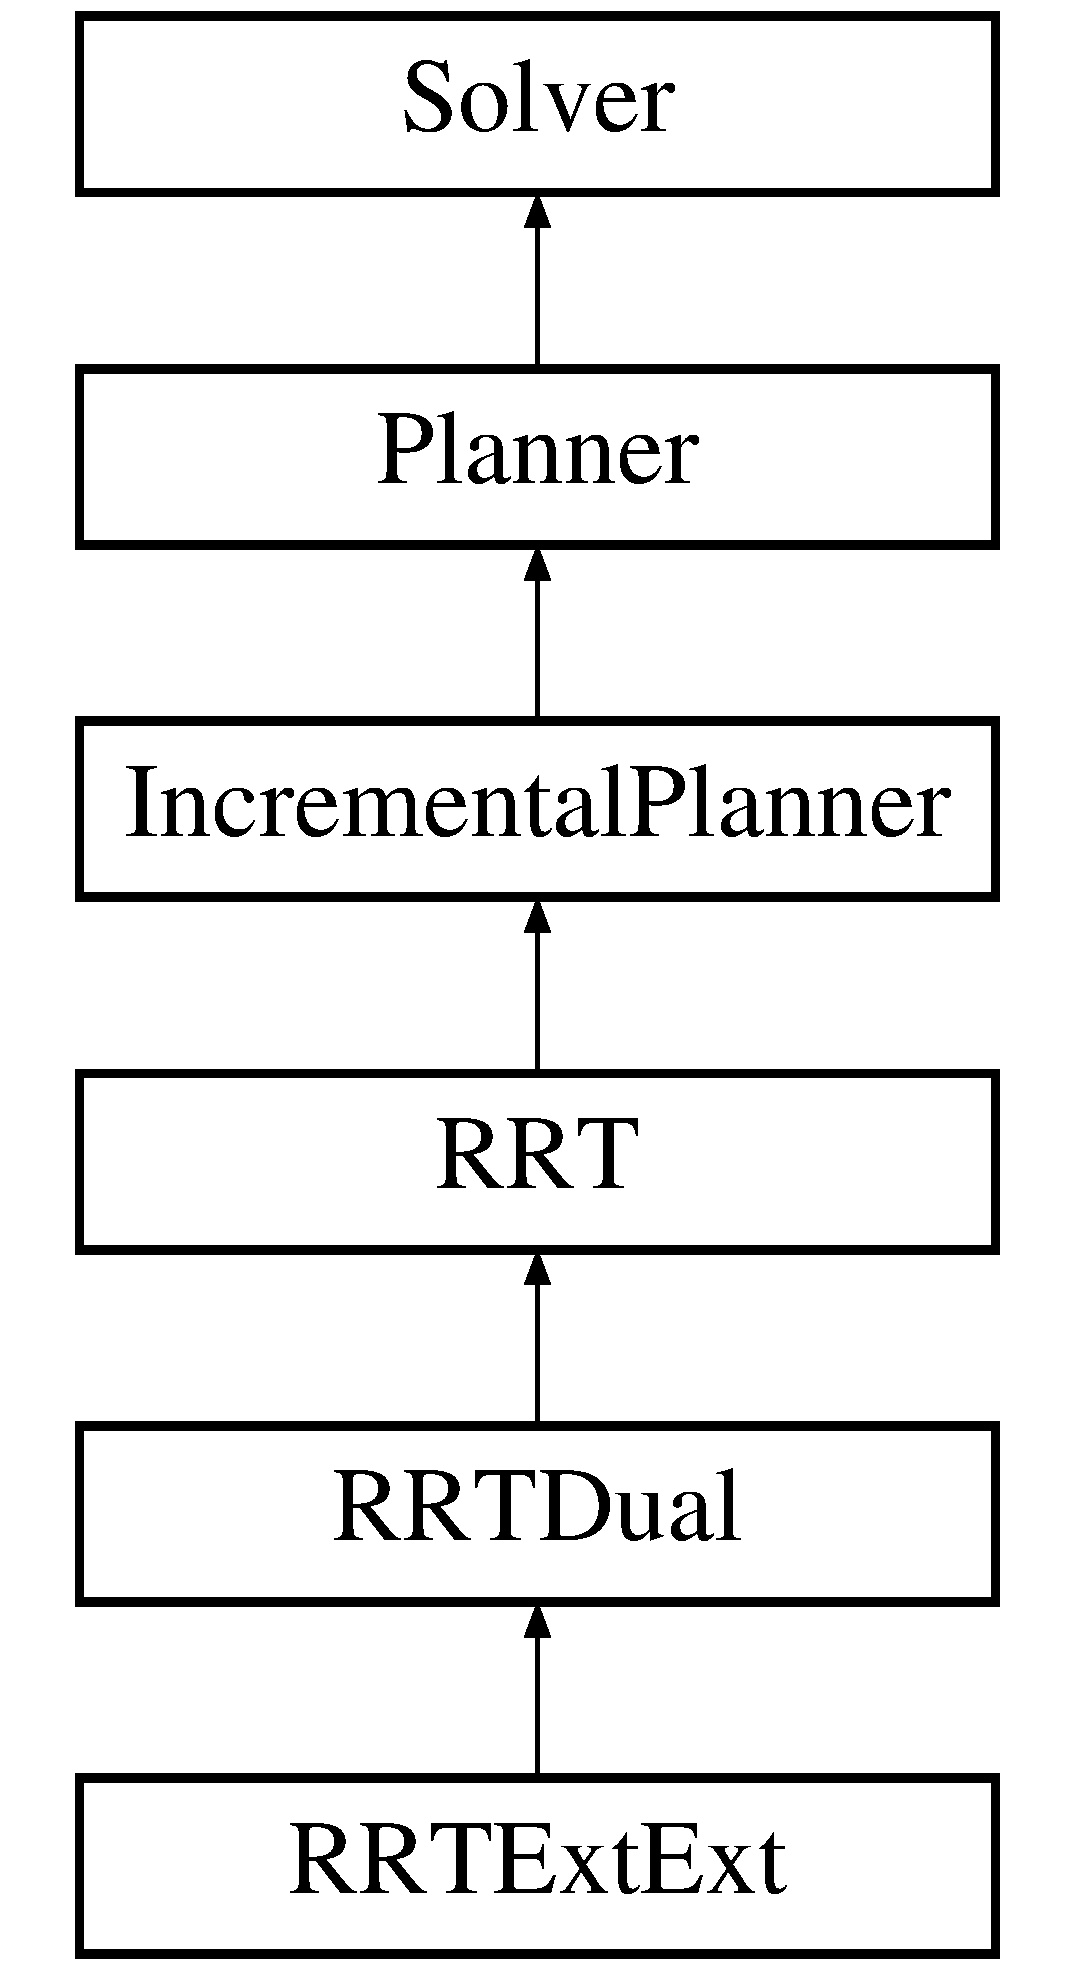
\includegraphics[height=6cm]{classRRTExtExt}
\end{center}
\end{figure}
\subsection*{Public Methods}
\begin{CompactItemize}
\item 
{\bf RRTExt\-Ext} ({\bf Problem} $\ast$p)
\item 
virtual {\bf $\sim$RRTExt\-Ext} ()
\item 
virtual bool {\bf Plan} ()
\begin{CompactList}\small\item\em The dual-tree planner used in La\-Valle, Kuffner, ICRA 1999. Each tree is extended toward a randomly-sampled point. RRTExt\-Ext is generally better.\item\end{CompactList}\end{CompactItemize}


\subsection{Detailed Description}
Balance between growing trees toward each other and exploring.

This planner balances the computation between growing the trees toward random samples and toward each other. G is the tree from the initial state, and G2 is the tree from the goal state. In each iteration, there are four steps: \begin{enumerate}
\item 
Use Extend to grow G toward a random sample \item 
Use Extend to grow G2 toward the new node in G \item 
Use Extend to grow G2 toward a random sample \item 
Use Extend to grow G toward the new node in G2 \end{enumerate}
In each step, node selection is based on the nearest neighbor. 



\subsection{Constructor \& Destructor Documentation}
\index{RRTExtExt@{RRTExt\-Ext}!RRTExtExt@{RRTExtExt}}
\index{RRTExtExt@{RRTExtExt}!RRTExtExt@{RRTExt\-Ext}}
\subsubsection{\setlength{\rightskip}{0pt plus 5cm}RRTExt\-Ext::RRTExt\-Ext ({\bf Problem} $\ast$ {\em p})}\label{classRRTExtExt_a0}


\index{RRTExtExt@{RRTExt\-Ext}!~RRTExtExt@{$\sim$RRTExtExt}}
\index{~RRTExtExt@{$\sim$RRTExtExt}!RRTExtExt@{RRTExt\-Ext}}
\subsubsection{\setlength{\rightskip}{0pt plus 5cm}virtual RRTExt\-Ext::$\sim$RRTExt\-Ext ()\hspace{0.3cm}{\tt  [inline, virtual]}}\label{classRRTExtExt_a1}




\subsection{Member Function Documentation}
\index{RRTExtExt@{RRTExt\-Ext}!Plan@{Plan}}
\index{Plan@{Plan}!RRTExtExt@{RRTExt\-Ext}}
\subsubsection{\setlength{\rightskip}{0pt plus 5cm}bool RRTExt\-Ext::Plan ()\hspace{0.3cm}{\tt  [virtual]}}\label{classRRTExtExt_a2}


The dual-tree planner used in La\-Valle, Kuffner, ICRA 1999. Each tree is extended toward a randomly-sampled point. RRTExt\-Ext is generally better.



Reimplemented from {\bf RRTDual} {\rm (p.\,\pageref{classRRTDual_a2})}.

The documentation for this class was generated from the following files:\begin{CompactItemize}
\item 
{\bf rrt.h}\item 
{\bf rrt.C}\end{CompactItemize}
